\documentclass[conference]{IEEEtran}
\IEEEoverridecommandlockouts

% Essential Packages
\usepackage{cite}
\usepackage{amsmath,amssymb,amsfonts}
\usepackage{algorithmic}
\usepackage{graphicx}
\usepackage{textcomp}
\usepackage{xcolor}
\usepackage{booktabs}
\usepackage{multirow}
\usepackage{tikz}
\usetikzlibrary{shapes.geometric, arrows, positioning, fit, calc}
\usepackage{url}

% Tighten bibliography item spacing to ensure all 12 references fit cleanly on page 8
\makeatletter
\def\thebibliography#1{\section*{\refname}%
    \addcontentsline{toc}{section}{\refname}%
    \footnotesize\vskip 0pt%
    \list{\@biblabel{\@arabic\c@enumiv}}%
    {\settowidth\labelwidth{\@biblabel{#1}}%
    \leftmargin\labelwidth
    \advance\leftmargin\labelsep
    \usecounter{enumiv}%
    \let\p@enumiv\@empty
    \renewcommand\theenumiv{\@arabic\c@enumiv}}%
    \def\IEEEbibitemsep{-0.5pt}%
    \sloppy\clubpenalty4000\widowpenalty4000\interlinepenalty500%
    \sfcode`\.=1000\relax}
\makeatother

\def\BibTeX{{\rm B\kern-.05em{\sc i\kern-.025em b}\kern-.08em
    T\kern-.1667em\lower.7ex\hbox{E}\kern-.125emX}}

\begin{document}

\title{A Validation-Aware and Evidence-Grounded AI Agent for Indoor Navigation Using TurtleBot3}

\author{
    \IEEEauthorblockN{
        Zhi-Heng Chen (7115064009),
        Cheng-Hao Hsiao (7115064186),
        Rui-Yu Lin (7115064168), \\
        Yuan-Mei Chiu (7115064159), and
        Yi-Kai Guan (7115093001)
    }
    \IEEEauthorblockA{
        \textit{Group 7, TurtleBot3 Project Team}
    }
}

\maketitle

\begin{abstract}
Language-controlled mobile robot navigation requires a system that correctly interprets natural language user commands, rigorously validates whether navigation is physically feasible under current robot conditions, executes goals reliably, and reports outcomes strictly grounded in observable operational evidence. Existing integrations of Large Language Models (LLMs) with ROS~2 navigation stacks primarily focus on semantic parsing efficiency or simulation latency, frequently overlooking the incremental contributions of interactive task clarification, pre-dispatch robot-state validation, and evidence-grounded reporting on a physical mobile platform. This paper presents the architecture, methodology, and planned evaluation protocol for a validation-aware AI agent operating on a physical TurtleBot3 Burger running Ubuntu 22.04 LTS, ROS~2 Humble, and Nav2. The proposed agent accepts Chinese-language task commands, parses intent using an LLM constrained by a strict JSON schema and registered landmark allowlist, performs pre-dispatch checks across sensor freshness, localization validity, and path feasibility, dispatches validated goals to Nav2, and produces user-facing reports derived exclusively from Nav2 terminal action outcomes and a tamper-resistant event log. To rigorously isolate the agent's contribution from the underlying navigation stack, three controlled baseline conditions are defined: B0 (fixed menu, Nav2 only), B1 (LLM with schema and allowlist, without clarification or pre-checks), and B2 (full validation-aware agent), alongside two ablation configurations. The experimental design encompasses 60 Chinese-language task cases (20 development / 40 test), 40 simulation runs per baseline method, and 12 paired physical robot navigation trials per method. Crucially, all experimental results presented in this paper represent planned evaluation protocols and expected research outcomes; no physical experiments have yet been executed, maintaining strict academic integrity.
\end{abstract}

\begin{IEEEkeywords}
indoor navigation, language-controlled robotics, ROS 2, Nav2, TurtleBot3, large language models, task clarification, evidence-grounded reporting, reliability evaluation.
\end{IEEEkeywords}

\section{Introduction}

The convergence of Large Language Models (LLMs) and autonomous robotic systems has established a promising paradigm for natural human-robot interaction in mobile robotics \cite{Yao2023react, Ahn2022saycan}. In indoor service and laboratory environments, natural language interfaces enable non-expert users to dispatch complex spatial tasks using intuitive phrases (e.g., in Mandarin Chinese, ``Please go to the experiment table'' [\textit{qing qu shi yan zhuo}] or ``Take me to the door'' [\textit{dai wo qu men kou}]) without needing to memorize specific coordinates, system menus, or domain-specific command syntax.

However, interpreting natural language alone does not guarantee reliable or safe physical robot operation. Physical mobile robot navigation in constrained indoor environments is fundamentally governed by real-world physical and sensor uncertainties:
\begin{enumerate}
    \item \textit{Wheel slippage and odometric divergence}: Differential-drive robots like the TurtleBot3 Burger accumulate significant odometry drift when wheels slip on low-friction floors or when the chassis is physically wedged against an obstacle while wheels continue to spin.
    \item \textit{Planar sensing limitations}: Standard 2D LiDAR sensors scan a single horizontal plane at a fixed elevation, rendering tabletop surfaces, hanging cables, and obstacles above or below the scan plane invisible.
    \item \textit{Geometric footprint inflation}: Nav2's global costmap inflates physical obstacles by the robot's footprint radius; narrow doorways that appear passable along a geometric centre-line may be rejected by the path planner due to conservative inflation margins.
    \item \textit{Localization filter latency}: Adaptive Monte Carlo Localization (AMCL) estimates may diverge or become stale without immediate diagnostic alerts in high-level task planners.
\end{enumerate}

When an unconstrained LLM directly commands a mobile robot, hallucinated coordinates, misunderstood landmark names, or dispatches initiated while the robot is unlocalized can lead to navigation failures, collisions, or unsupported claims of mission success. Recent integrations of LLMs with ROS~2 architectures, such as the work by Pollini et al. \cite{Pollini2025latency}, have explored latency reduction in command interpretation in simulation. However, these systems do not systematically investigate the incremental reliability and safety benefits introduced by interactive task clarification, pre-dispatch state and path validation, and evidence-grounded reporting on a physical mobile robot.

To address this gap, this paper introduces a \textit{validation-aware and evidence-grounded AI agent} designed for indoor navigation on the TurtleBot3 Burger platform. The system operates hierarchically above the ROS~2 Humble and Nav2 stack. The agent parses user commands into schema-constrained structured intents, verifies targets against an authoritative Landmark Registry, executes thorough pre-dispatch checks (sensor freshness, TF transform continuity, and global path feasibility), dispatches validated actions through a custom Navigation Adapter, and delivers mission reports strictly tied to Nav2 action results and an event audit log.

Three core research questions drive our investigation:
\begin{itemize}
    \item \textbf{RQ1 (Task Reliability)}: Does interactive task clarification combined with pre-dispatch robot state and path validation significantly reduce the rate of improper goal dispatch compared to unvalidated baselines?
    \item \textbf{RQ2 (Reporting Accuracy)}: Does evidence-grounded reporting eliminate unsupported success claims and improve consistency between reported status and physical robot outcomes?
    \item \textbf{RQ3 (Interaction Latency)}: What additional computational and communication latency does the full validation-aware agent introduce across the command-to-dispatch and dispatch-to-completion pipelines?
\end{itemize}

\textit{Academic Integrity Statement}: This paper documents a comprehensive system architecture, formal specification, and rigorous experimental protocol. In strict adherence to academic research integrity, all quantitative evaluation tables and performance figures presented herein reflect planned methodologies and expected experimental outcomes. No physical robot runs have been completed at this stage, and no synthetic empirical data have been fabricated.

The remainder of this paper is structured as follows. Section~II reviews related literature, outlines three core research debates, and presents a comparative literature matrix. Section~III details the eight-module, three-layer system architecture and core robotics design principles. Section~IV presents the methodology, task workflow, and exception-handling logic. Section~V outlines the experimental protocol, baseline conditions, ablations, and metric definitions. Section~VI discusses expected evaluation outcomes and failure preservation protocols. Section~VII concludes the paper and outlines future milestones.

\section{Related Work}

\subsection{LLM Reasoning and Robotic Tool Grounding}
Recent advances in natural language processing have demonstrated that LLMs can function as high-level task planners. Yao et al. \cite{Yao2023react} introduced the ReAct paradigm, wherein language models interleave reasoning traces with domain-specific tool invocations, updating internal state based on observation streams. Ahn et al. \cite{Ahn2022saycan} demonstrated SayCan, which grounds language plans in physical robot affordances by evaluating skill feasibility value functions on a mobile manipulation platform. In the ROS~2 domain, Pollini et al. \cite{Pollini2025latency} evaluated latency characteristics when connecting ChatGPT with a ROS~2 navigation framework in Gazebo simulation. While these works show the potential of tool-calling LLMs, they either target text environments \cite{Yao2023react}, specialized manipulation platforms \cite{Ahn2022saycan}, or simulation setups without evaluating physical pre-dispatch validation or landmark ambiguity clarification \cite{Pollini2025latency}.

\subsection{Modular Navigation and Mapping in ROS 2}
The open-source ROS~2 ecosystem provides robust, production-grade navigation and localization infrastructure. Macenski et al. \cite{Macenski2020marathon2} introduced the Marathon 2 Navigation System (Nav2), utilizing a behavior-tree architecture to coordinate global planners, local trajectory controllers, costmaps, and recovery behaviors. Macenski and Jambrecic \cite{Macenski2021slamtoolbox} developed SLAM Toolbox, offering lifelong mapping and optimization-based pose-graph localization in dynamic indoor environments. These components provide the foundational execution layer for our work. However, Nav2 and SLAM Toolbox operate purely on geometric coordinates and costmaps; they possess no inherent mechanisms for interpreting semantic Chinese text, resolving landmark ambiguities, or enforcing pre-dispatch validation rules prior to action dispatch.

\subsection{Navigation Reliability in Constrained Environments}
Evaluating mobile robot reliability in tightly constrained environments has received heightened attention. Xiao et al. \cite{Xiao2022barn} established the Benchmark Autonomous Robot Navigation (BARN) Challenge at ICRA, evaluating classical and learning-based planners across complex physical and simulated obstacle fields. Similarly, El-Hariry et al. \cite{ElHariry2025navbench} introduced NavBench, standardizing cross-platform reinforcement learning evaluations. The ongoing BARN Challenge 2026 \cite{Xiao2026barn} further underscores the unresolved nature of navigating dense spaces without collisions. These benchmarks highlight that navigation reliability depends heavily on footprint-to-gap ratios, costmap inflation parameters, and sensor coverage limitations.

\begin{table*}[t]
\caption{Related Work and Capability Comparison}
\label{tab:related_work}
\centering
\scriptsize
\setlength{\tabcolsep}{3.5pt}
\begin{tabular}{p{2.3cm}p{2.4cm}p{2.1cm}p{1.9cm}p{2.2cm}p{2.2cm}p{1.9cm}}
\toprule
\textbf{Approach / Reference} & \textbf{Focus / Method} & \textbf{Target Platform} & \textbf{Chinese NL Parsing} & \textbf{Pre-Dispatch State Check} & \textbf{Evidence-Grounded Reporting} & \textbf{Controlled Isolation} \\
\midrule
ReAct \cite{Yao2023react} & Reasoning + Actions & Text / Virtual Web & No & No & Partial & No \\
SayCan \cite{Ahn2022saycan} & Affordance Grounding & Mobile Manipulator & No & Skill Affordance & No & No \\
Pollini et al. \cite{Pollini2025latency} & LLM-ROS~2 Latency & Gazebo Mobile Robot & No & No & No & No \\
Nav2 \cite{Macenski2020marathon2} & Modular Navigation & Mobile Ground Robots & N/A & Internal Recovery & No & Fixed Substrate \\
SLAM Toolbox \cite{Macenski2021slamtoolbox} & Mapping / Localization & Mobile Robots & N/A & Scan Matching / Odom & N/A & N/A \\
BARN \cite{Xiao2022barn, Xiao2026barn} & Constrained Benchmark & Clearpath Jackal & N/A & Costmap Collision & No & Benchmark \\
NavBench \cite{ElHariry2025navbench} & RL Navigation Bench & Wheeled Robots / Sim & N/A & Policy Space & No & Benchmark \\
\textbf{Proposed System} & \textbf{Validation-Aware Agent} & \textbf{TurtleBot3 Burger} & \textbf{Yes} & \textbf{Yes (Freshness, TF, Path)} & \textbf{Yes (Nav2 Action Log)} & \textbf{Yes (Fixed Nav2)} \\
\bottomrule
\end{tabular}
\end{table*}

\subsection{Research Debates and Design Positioning}
Three central debates in robotic navigation directly informed our architectural decisions:
\begin{enumerate}
    \item \textit{Modular vs. End-to-End Navigation}: Modular architectures (Nav2) provide explicit boundaries for localization, planning, and control, allowing isolated debugging and determinism \cite{Macenski2020marathon2}. End-to-end learned policies map observations directly to control actions \cite{ElHariry2025navbench}, offering adaptive potential but suffering from opacity and unverified safety boundaries in narrow spaces. \textit{Our Positioning}: We fix Nav2 as an invariant navigation substrate across all evaluation conditions, isolating the AI agent as the sole experimental variable.
    \item \textit{Map-Based vs. Mapless Navigation}: Map-based systems rely on pre-built occupancy grids to compute global shortest paths and resolve semantic landmarks. Mapless reactive controllers avoid mapping overhead but cannot reason over named destinations or verify path feasibility prior to dispatch. \textit{Our Positioning}: We employ a pre-built 2D occupancy grid, an authoritative Landmark Registry, and dynamic local costmaps.
    \item \textit{Safety Margins vs. Traversability Efficiency}: Inflating obstacle safety margins minimizes collision risk under localization drift but renders narrow corridors geometrically impassable to the global planner \cite{Nav2TuningGuide}. Aggressive parameters preserve traversability but increase collision vulnerability \cite{Xiao2022barn}. \textit{Our Positioning}: We hold empirically validated Nav2 costmap parameters constant across all baselines, evaluating arrival rates, collision counts, and elapsed times simultaneously.
\end{enumerate}

Table~\ref{tab:related_work} contrasts the proposed architecture against existing representative literature across key functional capabilities.

\section{Proposed System Architecture}

\subsection{Platform and Operational Constraints}
The system targets a physical TurtleBot3 Burger mobile robot operating in a structured indoor laboratory environment \cite{RobotisTurtlebot3}. The platform specifications are summarized as follows:
\begin{itemize}
    \item \textbf{Robot Platform}: TurtleBot3 Burger (differential drive, wheel radius 33\,mm, track width 160\,mm) \cite{RobotisTurtlebot3}.
    \item \textbf{Compute and Middleware}: Onboard single-board computer running Ubuntu 22.04 LTS and ROS~2 Humble Hawksbill.
    \item \textbf{Primary Sensor}: 360$^\circ$ planar 2D LiDAR (LDS-01/02), scanning at 5\,Hz on a horizontal plane at an elevation of 145\,mm \cite{RobotisTurtlebot3}.
    \item \textbf{Localization and Navigation}: AMCL pose estimation coupled with Nav2 behaviour-tree navigation on a pre-built 2D occupancy grid ($0.05\,\text{m}/\text{pixel}$).
    \item \textbf{Scope Boundaries}: Single-floor planar navigation, pre-registered static landmarks, and Chinese-language commands. Multi-floor elevation, dynamic destination registration, and direct motor control from the LLM are strictly out of scope.
\end{itemize}

\begin{figure}[t]
\centering
% Figure 1: Overall System Architecture (8 Modules, 3 Layers)
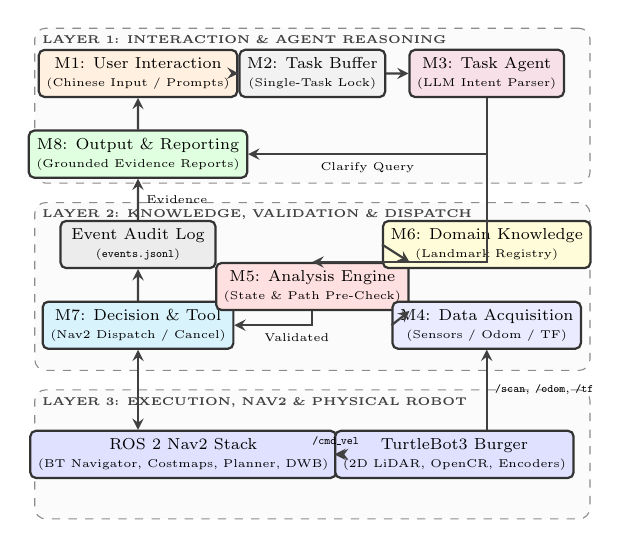
\begin{tikzpicture}[
    scale=0.82, every node/.style={transform shape},
    box/.style={rectangle, draw=black!80, fill=blue!5, thick, rounded corners=2pt, minimum width=2.3cm, minimum height=0.72cm, align=center, font=\scriptsize},
    layer/.style={rectangle, draw=black!45, dashed, fill=gray!3, rounded corners=4pt, inner sep=5pt},
    arr/.style={->, >=stealth, thick, draw=black!75},
    biarr/.style={<->, >=stealth, thick, draw=black!75},
    lbl/.style={font=\tiny\bfseries, text=black!75}
]

% ================= LAYER 1: INTERACTION & AGENT REASONING =================
\node[layer, minimum width=8.6cm, minimum height=2.4cm] (l1) at (0, 3.5) {};
\node[lbl, anchor=north west] at (l1.north west) {LAYER 1: INTERACTION \& AGENT REASONING};

\node[box, fill=orange!12, minimum width=2.4cm] (m1) at (-2.7, 4.0) {M1: User Interaction\\ \tiny (Chinese Input / Prompts)};
\node[box, fill=gray!10,   minimum width=2.2cm] (m2) at (0.0, 4.0)  {M2: Task Buffer\\ \tiny (Single-Task Lock)};
\node[box, fill=purple!12, minimum width=2.3cm] (m3) at (2.7, 4.0)  {M3: Task Agent\\ \tiny (LLM Intent Parser)};
\node[box, fill=green!12,  minimum width=2.4cm] (m8) at (-2.7, 2.75) {M8: Output \& Reporting\\ \tiny (Grounded Evidence Reports)};

\draw[arr] (m1) -- (m2);
\draw[arr] (m2) -- (m3);
\draw[arr] (m3.south) |- node[below, font=\tiny, pos=0.75]{Clarify Query} (m8.east);
\draw[arr] (m8) -- (m1);

% ================= LAYER 2: KNOWLEDGE, VALIDATION & DISPATCH =================
\node[layer, minimum width=8.6cm, minimum height=2.6cm] (l2) at (0, 0.7) {};
\node[lbl, anchor=north west] at (l2.north west) {LAYER 2: KNOWLEDGE, VALIDATION \& DISPATCH};

\node[box, fill=gray!15,   minimum width=2.4cm] (log) at (-2.7, 1.35) {Event Audit Log\\ \tiny (\texttt{events.jsonl})};
\node[box, fill=cyan!15,   minimum width=2.4cm] (m7)  at (-2.7, 0.1)  {M7: Decision \& Tool\\ \tiny (Nav2 Dispatch / Cancel)};
\node[box, fill=red!12,    minimum width=2.4cm] (m5)  at (0.0, 0.7)   {M5: Analysis Engine\\ \tiny (State \& Path Pre-Check)};
\node[box, fill=yellow!15, minimum width=2.4cm] (m6)  at (2.7, 1.35)  {M6: Domain Knowledge\\ \tiny (Landmark Registry)};
\node[box, fill=blue!8,    minimum width=2.4cm] (m4)  at (2.7, 0.1)   {M4: Data Acquisition\\ \tiny (Sensors / Odom / TF)};

% Layer 2 intra-flows
\draw[arr] (m3.south) |- (m5.north);
\draw[arr] (m6.west) -- (m5.north east);
\draw[arr] (m4.west) -- (m5.south east);
\draw[arr] (m5.south) |- node[below, font=\tiny, pos=0.6]{Validated} (m7.east);
\draw[arr] (m7) -- (log);
\draw[arr] (log) -- node[right, font=\tiny]{Evidence} (m8);

% ================= LAYER 3: EXECUTION, NAV2 & PHYSICAL ROBOT =================
\node[layer, minimum width=8.6cm, minimum height=2.0cm] (l3) at (0, -1.9) {};
\node[lbl, anchor=north west] at (l3.north west) {LAYER 3: EXECUTION, NAV2 \& PHYSICAL ROBOT};

\node[box, fill=blue!12, minimum width=3.4cm] (nav) at (-2.0, -1.9) {ROS 2 Nav2 Stack\\ \tiny (BT Navigator, Costmaps, Planner, DWB)};
\node[box, fill=blue!12, minimum width=3.0cm] (tb3) at (2.2, -1.9)  {TurtleBot3 Burger\\ \tiny (2D LiDAR, OpenCR, Encoders)};

% Inter-layer execution connections
\draw[biarr] (m7.south) -- (m7.south |- nav.north);
\draw[biarr] (nav) -- node[above, font=\tiny]{\texttt{/cmd\_vel}} (tb3);
\draw[arr]   (tb3.north -| m4.south) -- node[right, font=\tiny]{\texttt{/scan}, \texttt{/odom}, \texttt{/tf}} (m4.south);

\end{tikzpicture}

\caption{Overall system architecture illustrating the three hierarchical layers, eight functional modules (M1--M8), and interaction with ROS~2 Humble Nav2.}
\label{fig:arch}
\end{figure}

\subsection{Three-Layer, Eight-Module Architecture}
As depicted in Fig.~\ref{fig:arch}, the system is organized into eight dedicated modules distributed across three hierarchical layers:

\subsubsection{Layer 1: Interaction and Agent Reasoning}
\begin{itemize}
    \item \textbf{Module 1 (User Interaction)}: Interacts with the robot via Mandarin Chinese natural language text, submitting task requests, providing disambiguation clarifications, or issuing urgent cancellations.
    \item \textbf{Module 2 (Task Input Buffer)}: Ingests incoming user strings, assigns unique message identifiers, and buffers requests under a strict single-task execution lock.
    \item \textbf{Module 3 (Task Agent / LLM)}: Houses the core LLM intent parser. It maps natural language into constrained JSON tool calls against an allowed tool schema. It is strictly prohibited from generating raw velocities or arbitrary coordinates.
    \item \textbf{Module 8 (Output and Reporting)}: Synthesizes user-facing status messages, formulating structured clarification inquiries or delivering terminal mission reports grounded in physical execution evidence.
\end{itemize}

\subsubsection{Layer 2: Knowledge, Validation, and Tool Dispatch}
\begin{itemize}
    \item \textbf{Module 4 (Data Acquisition)}: Continuously subscribes to ROS~2 telemetry, aggregating LaserScan messages (\texttt{/scan}), wheel odometry (\texttt{/odom}), localization estimates (\texttt{/amcl\_pose}), and the TF2 transform tree (\texttt{map} $\to$ \texttt{odom} $\to$ \texttt{base\_link}).
    \item \textbf{Module 5 (Analysis Engine)}: Executes pre-dispatch safety and state checks. It evaluates sensor data age against freshness thresholds, verifies TF continuity and localization covariance, and queries the Nav2 global planner for geometric path feasibility.
    \item \textbf{Module 6 (Domain Knowledge)}: Maintains the authoritative Landmark Registry (\texttt{landmarks.json}), semantic Chinese aliases, forbidden operational zones, and tool parameter schemas.
    \item \textbf{Module 7 (Decision and Tool Dispatch)}: Manages navigation action lifecycles. It interfaces directly with Nav2 action servers through a Navigation Adapter, monitors feedback, tracks execution timeouts, enforces cancellation requests, and appends structured records to an immutable event audit log (\texttt{events.jsonl}).
\end{itemize}

\subsubsection{Layer 3: Execution, Nav2, and Physical Robot}
\begin{itemize}
    \item \textbf{ROS~2 Nav2 Stack}: Houses the modular navigation pipeline, including the Behavior Tree Navigator, NavFn/Smac Global Planner, DWB Local Controller, Costmap2D obstacle layers, Collision Monitor \cite{Nav2CollisionMonitor}, and recovery plugins.
    \item \textbf{TurtleBot3 Hardware}: Executes closed-loop differential motor control via the OpenCR microcontroller and streams planar LiDAR distance arrays \cite{RobotisTurtlebot3}.
\end{itemize}

\subsection{Governing Design Principles}
The architectural separation of concerns is grounded in five core engineering principles established in mobile robotics:
\begin{enumerate}
    \item \textit{Localization Uncertainty}: Position belief is a probabilistic estimate subject to drift. The agent must verify that AMCL localization covariance is within bounds and that the TF chain is active before dispatching goals.
    \item \textit{Sensor Limitations}: 2D LiDAR cannot detect obstacles above or below its horizontal scan plane. The system enforces sensor freshness thresholds ($\Delta t < 1.0\,\text{s}$) to prevent dispatching goals using stale sensor data, and transparently discloses planar blind spots \cite{RobotisTurtlebot3}.
    \item \textit{Physical Navigation Feasibility}: Paths must accommodate the robot's physical circular footprint. If Nav2's global planner cannot generate a collision-free path under configured footprint inflation, the agent rejects dispatch with \texttt{NO\_PATH}.
    \item \textit{Hierarchical Separation of Control}: Real-time obstacle avoidance demands millisecond-scale reactive loops, whereas LLM reasoning incurs hundreds of milliseconds of latency. Therefore, real-time safety remains exclusively within Nav2's local controller and collision monitor \cite{Nav2CollisionMonitor}; the LLM never executes real-time motor control loops.
    \item \textit{Reproducible Reliability Evaluation}: True system reliability cannot be inferred from cherry-picked successful trials. All failures, timeouts, and anomalies must be captured in immutable event logs and fully reported.
\end{enumerate}

\section{Methodology and Task Workflow}

\subsection{Chinese Natural Language Intent Parsing}
When a Chinese text command is ingested by Module~2, the Task Agent (Module~3) parses the utterance into a structured intent matching a rigid JSON schema:
\begin{equation}
\label{eq:intent}
\begin{aligned}
\mathcal{I} = \{ & \text{intent}: \texttt{navigate} \mid \texttt{cancel} \mid \texttt{query}, \\
& \text{landmark\_id}: \text{string} \}
\end{aligned}
\end{equation}
The prompt explicitly binds the output space to allowed tool names and registered landmark identifiers. Any command attempting to inject arbitrary Python code, raw velocity vectors, or unlisted destinations is immediately rejected by the schema validator.

\subsection{Landmark Registry and Ambiguity Clarification}
The Landmark Registry acts as the authoritative knowledge base, mapping natural Chinese names and aliases to registered poses $\mathbf{p} = (x, y, \theta)$ in the \texttt{map} frame:
\begin{equation}
\label{eq:landmark}
\mathcal{L} = \langle \text{id}, \text{name}, \mathcal{A}, (x, y, \theta)_{\text{map}} \rangle
\end{equation}
where $\mathcal{A}$ denotes the set of recognized natural language aliases. When parsed intent yields an unrecognized target, the agent returns \texttt{REJECTED}. Crucially, when an intent matches multiple distinct registered destinations (e.g., ``the door'' [\textit{men kou}] in a laboratory with both \texttt{door-north} and \texttt{door-south}), the agent transitions to \texttt{CLARIFY}. It halts dispatch and instructs Module~8 to present a disambiguation query to the user, strictly avoiding arbitrary guessing.

\begin{figure}[t]
\centering
% Figure 2: Validation-Dispatch-Monitoring Workflow
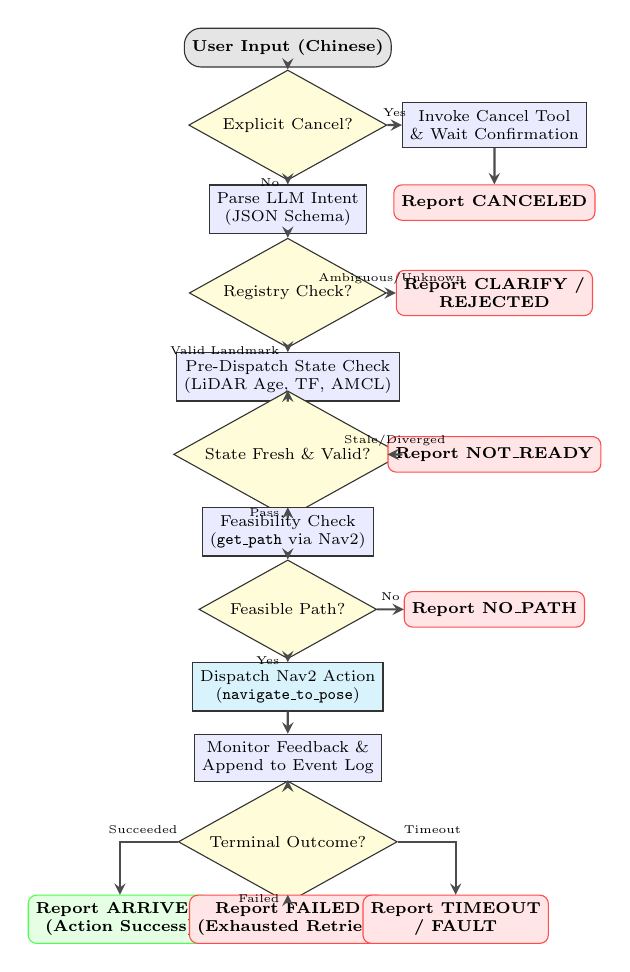
\begin{tikzpicture}[
    scale=0.82, every node/.style={transform shape},
    startstop/.style={rectangle, rounded corners=6pt, minimum width=2.4cm, minimum height=0.6cm, align=center, draw=black!80, fill=gray!20, font=\scriptsize\bfseries},
    process/.style={rectangle, minimum width=2.4cm, minimum height=0.65cm, align=center, draw=black!80, fill=blue!8, font=\scriptsize},
    decision/.style={diamond, aspect=1.8, minimum width=2.2cm, align=center, draw=black!80, fill=yellow!15, font=\scriptsize},
    arr/.style={->, >=stealth, thick, draw=black!70},
    fail/.style={rectangle, rounded corners=3pt, minimum width=1.8cm, minimum height=0.55cm, align=center, draw=red!70, fill=red!10, font=\scriptsize\bfseries},
    succ/.style={rectangle, rounded corners=3pt, minimum width=1.8cm, minimum height=0.55cm, align=center, draw=green!70, fill=green!10, font=\scriptsize\bfseries}
]

% Nodes
\node[startstop] (start) at (0, 0) {User Input (Chinese)};
\node[decision] (cancel) at (0, -1.2) {Explicit Cancel?};
\node[process] (do_cancel) at (3.2, -1.2) {Invoke Cancel Tool\\\& Wait Confirmation};
\node[fail] (res_cancel) at (3.2, -2.4) {Report CANCELED};

\node[process] (parse) at (0, -2.5) {Parse LLM Intent\\(JSON Schema)};
\node[decision] (allow) at (0, -3.8) {Registry Check?};
\node[fail] (clarify) at (3.2, -3.8) {Report CLARIFY /\\REJECTED};

\node[process] (sensor) at (0, -5.1) {Pre-Dispatch State Check\\(LiDAR Age, TF, AMCL)};
\node[decision] (valid) at (0, -6.3) {State Fresh \& Valid?};
\node[fail] (notready) at (3.2, -6.3) {Report NOT\_READY};

\node[process] (path) at (0, -7.5) {Feasibility Check\\(\texttt{get\_path} via Nav2)};
\node[decision] (path_ok) at (0, -8.7) {Feasible Path?};
\node[fail] (nopath) at (3.2, -8.7) {Report NO\_PATH};

\node[process, fill=cyan!15] (dispatch) at (0, -9.9) {Dispatch Nav2 Action\\(\texttt{navigate\_to\_pose})};
\node[process] (monitor) at (0, -11.0) {Monitor Feedback \&\\Append to Event Log};

\node[decision] (terminal) at (0, -12.3) {Terminal Outcome?};
\node[succ] (arrived) at (-2.6, -13.5) {Report ARRIVED\\(Action Success)};
\node[fail] (failed) at (0, -13.5) {Report FAILED\\(Exhausted Retries)};
\node[fail] (timeout) at (2.6, -13.5) {Report TIMEOUT\\/ FAULT};

% Arrows
\draw[arr] (start) -- (cancel);
\draw[arr] (cancel) -- node[above, font=\tiny]{Yes} (do_cancel);
\draw[arr] (do_cancel) -- (res_cancel);
\draw[arr] (cancel) -- node[left, font=\tiny]{No} (parse);

\draw[arr] (parse) -- (allow);
\draw[arr] (allow) -- node[above, font=\tiny]{Ambiguous/Unknown} (clarify);
\draw[arr] (allow) -- node[left, font=\tiny]{Valid Landmark} (sensor);

\draw[arr] (sensor) -- (valid);
\draw[arr] (valid) -- node[above, font=\tiny]{Stale/Diverged} (notready);
\draw[arr] (valid) -- node[left, font=\tiny]{Pass} (path);

\draw[arr] (path) -- (path_ok);
\draw[arr] (path_ok) -- node[above, font=\tiny]{No} (nopath);
\draw[arr] (path_ok) -- node[left, font=\tiny]{Yes} (dispatch);

\draw[arr] (dispatch) -- (monitor);
\draw[arr] (monitor) -- (terminal);

\draw[arr] (terminal) -| node[above, font=\tiny, pos=0.3]{Succeeded} (arrived);
\draw[arr] (terminal) -- node[left, font=\tiny]{Failed} (failed);
\draw[arr] (terminal) -| node[above, font=\tiny, pos=0.3]{Timeout} (timeout);

\end{tikzpicture}

\caption{Validation--Dispatch--Monitoring task execution workflow and state transition logic.}
\label{fig:workflow}
\end{figure}

\subsection{Pre-Dispatch Robot State and Path Validation}
Prior to issuing any navigation action to Nav2, Module~5 performs three mandatory pre-checks:
\begin{enumerate}
    \item \textit{Sensor Freshness Check}: Verifies that the timestamp of the latest \texttt{/scan} message satisfies $t_{\text{current}} - t_{\text{scan}} < \tau_{\text{sensor}}$ (with $\tau_{\text{sensor}} = 1.0\,\text{s}$). Stale scans indicate sensor failure or driver hang, yielding \texttt{NOT\_READY}.
    \item \textit{Localization and TF Continuity Check}: Verifies that the transform from \texttt{map} to \texttt{base\_link} exists and has been updated within $\tau_{\text{TF}} = 0.5\,\text{s}$, and that AMCL pose covariance matrix eigenvalues remain below an empirically established dispersion limit $\sigma^2_{\text{pose}} < \sigma^2_{\text{thresh}}$.
    \item \textit{Path Feasibility Check}: Invokes the Navigation Adapter's \texttt{get\_path} service (communicating with Nav2's \texttt{ComputePathToPose} action server). If the global costmap indicates that the target is inside an inflated obstacle zone or geometrically unreachable, the planner returns an empty path, prompting an immediate \texttt{NO\_PATH} report without motor activation.
\end{enumerate}

\subsection{Execution, Monitoring, and Exception Handling}
Upon successful validation, Module~7 dispatches a \texttt{NavigateToPose} action goal to Nav2. The complete lifecycle workflow is illustrated in Fig.~\ref{fig:workflow}. During execution, the system maintains a single-task lock.
\begin{itemize}
    \item \textit{Mid-Task Cancellation}: If the user issues an explicit cancel command (e.g., ``stop'' [\textit{ting zhi}] or ``cancel'' [\textit{qu xiao}]), the request bypasses LLM re-reasoning. Module~7 transmits a cancel goal request directly to the Nav2 action client \cite{Nav2SimpleCommander}. The agent monitors status until Nav2 confirms action termination, only then transitioning to \texttt{CANCELED}.
    \item \textit{Watchdog Timeout}: Each mission is assigned a maximum execution budget $T_{\text{max}} = 120\,\text{s}$. If Nav2 fails to achieve the goal within this window, the agent issues an abort and logs \texttt{TIMEOUT}.
    \item \textit{Qualified Single-Retry}: If Nav2 aborts due to a transient planner recovery failure, the agent verifies whether robot state remains valid and permits exactly one re-planning attempt before declaring \texttt{FAILED}.
\end{itemize}

\subsection{Evidence-Grounded Reporting}
Module~8 delivers the final report to the user. A strict architectural constraint governs success reporting:
\begin{equation}
\label{eq:evidence}
\begin{aligned}
\text{Report} = \texttt{ARRIVED} \iff & (\mathcal{S}_{\text{Nav2}} = \texttt{SUCCEEDED}) \\
& \land (\|\mathbf{p}_{\text{final}} - \mathbf{p}_{\text{target}}\| < \epsilon_{\text{dist}})
\end{aligned}
\end{equation}
If Nav2 reports failure, or if communication is lost, the agent is structurally incapable of asserting success. All mission events, error codes, and intermediate timestamps are appended to \texttt{events.jsonl}.

\section{Experimental Design}

\subsection{Baseline Condition Separation}
To rigorously isolate the incremental contribution of the agent layer, we define three controlled baseline conditions sharing an identical ROS~2 Humble and Nav2 navigation infrastructure (same costmap resolutions, inflation radii, and DWB trajectory generator settings):
\begin{itemize}
    \item \textbf{B0 (Fixed Menu Baseline)}: The robot is commanded via a pre-defined numeric menu (e.g., selecting ``Destination 1'' directly dispatches coordinates to Nav2). B0 evaluates Nav2's raw physical navigation capability in the absence of natural language parsing, clarification, or agent-level state validation.
    \item \textbf{B1 (Language Baseline)}: The robot accepts Chinese natural language commands. Intent is parsed using an LLM constrained by JSON schema and landmark allowlist. However, B1 lacks interactive ambiguity clarification (it defaults to the first coordinate match) and omits pre-dispatch sensor/path validation (goals are directly dispatched to Nav2).
    \item \textbf{B2 (Full Validation-Aware Agent)}: The proposed system, integrating Chinese language parsing, interactive ambiguity clarification, pre-dispatch state/path checks, execution monitoring, and evidence-grounded reporting.
\end{itemize}

In addition, two ablation variants isolate individual components:
\begin{itemize}
    \item \textbf{B2 $-$ Clarification}: Full agent omitting Module~8's clarification prompt on ambiguous inputs, evaluating the specific contribution of clarification to preventing improper dispatch.
    \item \textbf{B2 $-$ Agent Pre-Check}: Full agent omitting Module~5's sensor freshness and path feasibility pre-checks prior to dispatch, while retaining Nav2's internal safety costmaps.
\end{itemize}

Table~\ref{tab:baselines} delineates the functional capability matrix across all evaluated conditions.

\begin{table}[t]
\caption{Baseline and Ablation Capability Matrix}
\label{tab:baselines}
\centering
\scriptsize
\setlength{\tabcolsep}{2.0pt}
\begin{tabular}{@{}p{3.1cm}ccccc@{}}
\toprule
\textbf{Capability / Feature} & \textbf{B0} & \textbf{B1} & \textbf{B2} & \textbf{B2-C} & \textbf{B2-P} \\
\midrule
Nav2 Execution Stack & \checkmark & \checkmark & \checkmark & \checkmark & \checkmark \\
Chinese Language Interface & $\times$ & \checkmark & \checkmark & \checkmark & \checkmark \\
Schema-Constrained Intent & $\times$ & \checkmark & \checkmark & \checkmark & \checkmark \\
Landmark Registry Allowlist & $\times$ & \checkmark & \checkmark & \checkmark & \checkmark \\
Interactive Disambiguation & $\times$ & $\times$ & \checkmark & $\times$ & \checkmark \\
Sensor Freshness Validation & $\times$ & $\times$ & \checkmark & \checkmark & $\times$ \\
Localization / TF Continuity Check & $\times$ & $\times$ & \checkmark & \checkmark & $\times$ \\
Nav2 Path Feasibility Pre-Check & $\times$ & $\times$ & \checkmark & \checkmark & $\times$ \\
Mid-Task Cancellation Watchdog & $\times$ & $\times$ & \checkmark & \checkmark & \checkmark \\
Evidence-Grounded Reporting & $\times$ & $\times$ & \checkmark & \checkmark & \checkmark \\
\bottomrule
\multicolumn{6}{@{}p{\columnwidth}@{}}{\scriptsize Note: B2-C denotes B2$-$Clarification; B2-P denotes B2$-$Agent Pre-Check.}
\end{tabular}
\end{table}

\subsection{Planned Experiment Protocol}
The planned evaluation framework comprises three distinct experimental tracks, detailed in Table~\ref{tab:protocol}:

\begin{table*}[t]
\caption{Planned Experimental Protocol and Track Specifications}
\label{tab:protocol}
\centering
\scriptsize
\setlength{\tabcolsep}{3.5pt}
\begin{tabular}{p{2.2cm}p{3.2cm}p{2.6cm}p{2.5cm}p{5.0cm}}
\toprule
\textbf{Evaluation Track} & \textbf{Scope and Input Distribution} & \textbf{Sample Size / Split} & \textbf{Evaluated Methods} & \textbf{Environment / Platform Setup} \\
\midrule
\textbf{Track 1: Language Understanding} & 6 command categories: Explicit, Ambiguous, Unknown, Cancel, Compound, Out-of-Scope (10 cases each) & 60 Chinese task cases (20 Dev / 40 Test) & B1, B2, B2-Clar. (B0 marked N/A) & Offline evaluation harness; simulated prompt ingestion with ground-truth intent annotations. \\
\addlinespace[3pt]
\textbf{Track 2: Simulation Navigation} & 4 Gazebo worlds $\times$ 2 topological routes $\times$ 5 repetitions & 40 simulation trials per method (120 trials total) & B0, B1, B2 & ROS~2 Humble + Gazebo 11 on Ubuntu 22.04 LTS; TurtleBot3 Burger model with simulated 2D LiDAR. \\
\addlinespace[3pt]
\textbf{Track 3: Real-Robot Navigation} & 12 paired navigation task scenarios across standardized start-goal pairs & 12 paired trials per method (36 runs total) & B0, B1, B2 & Physical TurtleBot3 Burger in structured indoor laboratory floor; pre-built occupancy map. \\
\addlinespace[3pt]
\textbf{Track 4: Ablation Studies} & Ambiguous language tasks and obstructed/stale pre-check conditions & 20 selected test cases per ablation variant & B2-Clar., B2-Pre. & Paired comparative trials against full B2 in simulation and physical environment. \\
\bottomrule
\end{tabular}
\end{table*}

\begin{enumerate}
    \item \textit{Language Understanding Track}: A curated benchmark of 60 Chinese natural language task utterances divided equally across six categories (10 explicit commands, 10 ambiguous landmarks, 10 unknown locations, 10 mid-task cancellations, 10 compound commands, and 10 out-of-scope requests). The corpus is strictly split into 20 development cases (for prompt tuning) and 40 held-out test cases.
    \item \textit{Simulation Navigation Track}: Conducted in Gazebo simulation across four distinct indoor room configurations and two routes per room, with five randomized runs per route, totaling 40 simulation trials per baseline.
    \item \textit{Physical Robot Navigation Track}: Executed on the physical TurtleBot3 Burger across 12 standardized, paired indoor route scenarios (same initial pose, same target landmark), comparing B0, B1, and B2 under identical environmental conditions without inducing intentional collisions.
\end{enumerate}

\subsection{Evaluation Metrics and Mathematical Definitions}
To evaluate RQ1–RQ3, we define the following operational metrics, summarized in Table~\ref{tab:metrics}:
\begin{enumerate}
    \item \textit{Task Handling Accuracy ($A_{\text{task}}$)}: Proportion of tasks correctly processed (dispatched if valid, clarified if ambiguous, rejected if invalid):
    \begin{equation}
    A_{\text{task}} = \frac{N_{\text{correct}}}{N_{\text{total}}}
    \end{equation}
    \item \textit{Improper Dispatch Rate ($R_{\text{improper}}$)}: Proportion of invalid, ambiguous, or unfeasible tasks for which a physical navigation goal was erroneously dispatched:
    \begin{equation}
    R_{\text{improper}} = \frac{N_{\text{dispatched\_invalid}}}{N_{\text{total\_invalid}}}
    \end{equation}
    \item \textit{Reporting Accuracy ($A_{\text{report}}$)}: Consistency between the agent's user-facing report and physical Nav2 terminal execution evidence:
    \begin{equation}
    A_{\text{report}} = \frac{N_{\text{evidence\_consistent}}}{N_{\text{evaluable\_reports}}}
    \end{equation}
    \item \textit{Navigation Success Rate ($S_{\text{nav}}$)}: Proportion of validly dispatched missions in which the robot successfully arrived within $\epsilon_{\text{dist}} = 0.15\,\text{m}$ of the target pose:
    \begin{equation}
    S_{\text{nav}} = \frac{N_{\text{arrived}}}{N_{\text{dispatched\_valid}}}
    \end{equation}
    \item \textit{Segmented Interaction Latency}: Recorded via event log timestamps across three discrete intervals:
    \begin{itemize}
        \item $T_0 \to T_1$: Time from user command receipt to structured intent completion.
        \item $T_1 \to T_2$: Time from intent completion through state validation to Nav2 goal acceptance.
        \item $T_2 \to T_3$: Time from Nav2 goal acceptance to terminal action completion.
    \end{itemize}
\end{enumerate}

All proportional metrics are evaluated with trial sample sizes $n$ and reported alongside Wilson 95\% score confidence intervals. If zero collisions occur across $n$ runs, the outcome will be formally reported as $0/n$ (95\% CI: $0.0\% \text{--} x\%$) rather than an ungrounded claim of ``zero collision probability.''

\begin{table*}[t]
\caption{Operational Metrics and Evaluation Framework}
\label{tab:metrics}
\centering
\scriptsize
\begin{tabular}{p{3.2cm}p{1.2cm}p{4.8cm}p{2.2cm}p{3.8cm}}
\toprule
\textbf{Metric Name} & \textbf{Target RQ} & \textbf{Operational / Mathematical Definition} & \textbf{Evaluated Baselines} & \textbf{Data Source / Logged Event Anchor} \\
\midrule
Task Handling Accuracy & RQ1 & $N_{\text{correct}} / N_{\text{total}}$ across language test suite & B1, B2, Ablations (B0: N/A) & Evaluation runner ground-truth matching \\
Improper Dispatch Rate & RQ1 & $N_{\text{dispatched\_invalid}} / N_{\text{total\_invalid}}$ & B1, B2, B2$-$Clar., B2$-$Pre. & Goal dispatch callbacks on invalid tasks \\
Reporting Accuracy & RQ2 & $N_{\text{evidence\_consistent}} / N_{\text{evaluable\_reports}}$ & B1, B2 & Cross-check of user report vs. Nav2 result \\
Unsupported Success Claims & RQ2 & Count of \texttt{ARRIVED} reports lacking Nav2 \texttt{SUCCEEDED} & B1, B2 & Terminal action log audit \\
Navigation Success Rate & General & $N_{\text{arrived}} / N_{\text{dispatched\_valid}}$ & B0, B1, B2 & Nav2 terminal status (\texttt{SUCCEEDED}) \\
Observed Collision Count & General & Physical contact events observed during trial & B0, B1, B2 & Direct observer log + bumper/LiDAR log \\
Parsing Latency ($T_0 \to T_1$) & RQ3 & Duration from command input to intent parse & B1, B2 (B0: N/A) & Timestamps $t_{\text{recv}}$ and $t_{\text{parsed}}$ in event log \\
Validation Latency ($T_1 \to T_2$) & RQ3 & Duration from intent parse to Nav2 goal dispatch & B2 (B0, B1: minimal) & Timestamps $t_{\text{parsed}}$ and $t_{\text{dispatch}}$ in event log \\
Navigation Latency ($T_2 \to T_3$) & RQ3 & Duration from Nav2 goal acceptance to completion & B0, B1, B2 & Timestamps $t_{\text{dispatch}}$ and $t_{\text{term}}$ in event log \\
\bottomrule
\end{tabular}
\end{table*}

\section{Proposed Evaluation and Expected Outcomes}

\subsection{Expected Research Outcomes}
The proposed validation-aware agent is anticipated to demonstrate clear improvements in task reliability and reporting fidelity, accompanied by a quantifiable interaction latency trade-off:
\begin{itemize}
    \setlength{\itemsep}{1.5pt}
    \setlength{\parskip}{0pt}
    \setlength{\parsep}{0pt}
    \item \textbf{RQ1 (Improper Dispatch Mitigation)}: Baseline B1 is expected to exhibit an elevated improper dispatch rate when presented with ambiguous landmarks (e.g., arbitrarily navigating to \texttt{door-north} when the user specified ``the door'' [\textit{men kou}]) or unfeasible goals (dispatching goals into occupied furniture). In contrast, B2 is designed to eliminate improper dispatches on ambiguous commands via interactive clarification, and substantially reduce unfeasible dispatches via pre-dispatch path checking. The ablation B2$-$Clarification is expected to confirm that clarification specifically prevents ambiguous-goal dispatches.
    \item \textbf{RQ2 (Zero Unsupported Success Claims)}: When navigation is aborted by Nav2 due to dynamic obstacles or odometry drift, B1 systems relying purely on high-level LLM reasoning may falsely conclude mission success once a goal is accepted. In contrast, B2's strict evidence rule (Eq.~\ref{eq:evidence}) is designed to ensure complete consistency with Nav2 physical execution, preventing false-positive success claims.
    \item \textbf{RQ3 (Latency Decomposition)}: Incorporating LLM semantic parsing and pre-dispatch checks introduces computational overhead. Segment $T_0 \to T_1$ introduces LLM inference latency, while $T_1 \to T_2$ adds sensor freshness verification and Nav2 \texttt{get\_path} computation time. Because physical Nav2 navigation execution ($T_2 \to T_3$, typically tens of seconds) dominates total task duration, the incremental latency introduced by B2 represents a planned, quantified trade-off for physical reliability.
\end{itemize}

\begin{table*}[t]
\caption{Planned Analysis Framework for Physical and Simulation Evaluation}
\label{tab:planned_results}
\centering
\scriptsize
\setlength{\tabcolsep}{2.5pt}
\begin{tabular}{@{}p{3.8cm}cccccc@{}}
\toprule
\textbf{Experimental Condition} & \begin{tabular}[c]{@{}c@{}}\textbf{Sample}\\\textbf{Size ($n$)}\end{tabular} & \begin{tabular}[c]{@{}c@{}}\textbf{Task}\\\textbf{Acc. (\%)}\end{tabular} & \begin{tabular}[c]{@{}c@{}}\textbf{Improper}\\\textbf{Disp. (\%)}\end{tabular} & \begin{tabular}[c]{@{}c@{}}\textbf{Report}\\\textbf{Acc. (\%)}\end{tabular} & \begin{tabular}[c]{@{}c@{}}\textbf{Nav.}\\\textbf{Success (\%)}\end{tabular} & \begin{tabular}[c]{@{}c@{}}\textbf{Median Lat.}\\\textbf{$T_0 \to T_2$ (s)}\end{tabular} \\
\midrule
\multicolumn{7}{@{}l}{\textit{Planned Simulation Track (40 runs per condition)}} \\
\quad Baseline B0 (Fixed Menu)          & 40 & N/A     & N/A     & N/A     & ---$^*$ & ---$^*$ \\
\quad Baseline B1 (Language, No Checks) & 40 & ---$^*$ & ---$^*$ & ---$^*$ & ---$^*$ & ---$^*$ \\
\quad Baseline B2 (Full Agent)          & 40 & ---$^*$ & ---$^*$ & ---$^*$ & ---$^*$ & ---$^*$ \\
\addlinespace[1pt]
\multicolumn{7}{@{}l}{\textit{Planned Real-Robot Track (12 paired runs per condition)}} \\
\quad Baseline B0 (Fixed Menu)          & 12 & N/A     & N/A     & N/A     & ---$^*$ & ---$^*$ \\
\quad Baseline B1 (Language, No Checks) & 12 & ---$^*$ & ---$^*$ & ---$^*$ & ---$^*$ & ---$^*$ \\
\quad Baseline B2 (Full Agent)          & 12 & ---$^*$ & ---$^*$ & ---$^*$ & ---$^*$ & ---$^*$ \\
\addlinespace[1pt]
\multicolumn{7}{@{}l}{\textit{Planned Ablation Track (Test Corpus / Selected Routes)}} \\
\quad Baseline B2 $-$ Clarification     & 20 & ---$^*$ & ---$^*$ & ---$^*$ & ---$^*$ & ---$^*$ \\
\quad Baseline B2 $-$ Agent Pre-Check   & 20 & ---$^*$ & ---$^*$ & ---$^*$ & ---$^*$ & ---$^*$ \\
\bottomrule
\multicolumn{7}{@{}p{\textwidth}@{}}{\scriptsize $^*$Note: Values marked with ``---'' represent planned experimental metrics to be recorded upon protocol execution; no numerical data have been fabricated.} \\
\end{tabular}
\end{table*}

\subsection{Planned Analysis Framework}
Table~\ref{tab:planned_results} outlines the planned comparative analysis framework. In accordance with academic integrity guidelines, numerical values are explicitly presented as planned analysis fields rather than synthetic empirical measurements.

\subsection{Failure Mode Taxonomy and Preservation}
In compliance with Core Principle~5, all evaluation trials resulting in non-arrival will be classified and retained in public repository records under the following taxonomy:
\begin{itemize}
    \setlength{\itemsep}{0.8pt}
    \setlength{\parskip}{0pt}
    \setlength{\parsep}{0pt}
    \item \texttt{NOT\_READY}: Stale LiDAR data ($>1.0\,\text{s}$), missing TF transforms, or localization covariance exceeding threshold.
    \item \texttt{NO\_PATH}: Nav2 global planner unable to find a valid trajectory accommodating the robot footprint.
    \item \texttt{REJECTED}: Utterance references an unregistered landmark or requests disallowed control commands.
    \item \texttt{CLARIFY}: Command maps to multiple registered destinations, successfully triggering user disambiguation.
    \item \texttt{CANCELED}: Goal successfully halted following explicit user cancellation.
    \item \texttt{FAILED}: Nav2 aborted navigation due to unrecoverable obstacles or controller oscillation.
    \item \texttt{TIMEOUT}: Mission exceeded the 120\,s execution budget.
\end{itemize}
No failed run will be omitted or classified as an ``outlier'' without logged evidence, ensuring reproducible benchmarking.

\section{Conclusion and Future Work}

This paper presented the architecture, methodology, and experimental design for a validation-aware and evidence-grounded AI agent enabling Chinese-language indoor navigation on a TurtleBot3 Burger. By hierarchically separating high-level language reasoning from real-time navigation control, the system constrains LLM output via rigid JSON schemas, verifies targets against an authoritative Landmark Registry, executes strict pre-dispatch sensor and path feasibility checks, and ensures that all user-facing reports are strictly anchored in physical Nav2 execution evidence. The experimental protocol outlines a rigorous, controlled evaluation across 60 language cases, 40 simulation runs, and 12 paired real-robot trials across B0, B1, and B2 baselines. Future work will execute the planned experimental matrix on the physical TurtleBot3 platform, conduct fine-grained statistical significance testing across segmented latencies, investigate continuous SLAM map updates for dynamic environments, and explore multi-floor navigation extensions.

\bibliographystyle{IEEEtran}
\bibliography{references}

\end{document}
